<<<<<<< HEAD
\begin{figure}[t]
    \centering
    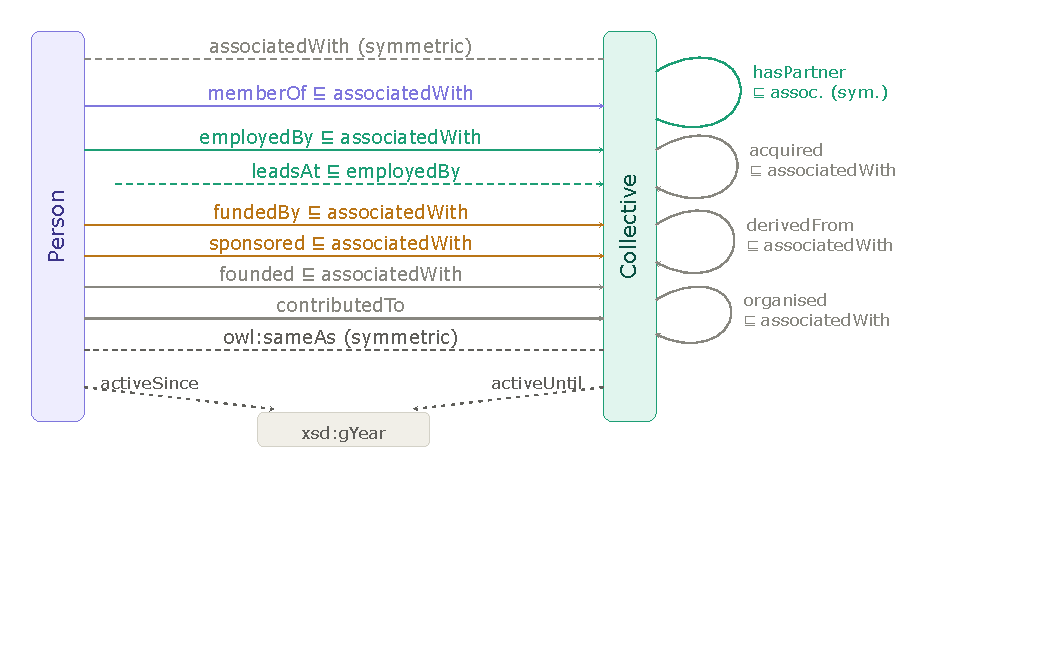
\includegraphics[trim={0 3.5cm 2cm 0cm},clip,width=\textwidth]{figures/lack-ontology-diagram.pdf}
    \vspace{-0.3cm}\caption{Schema diagram of the LACK ontology.}
\label{fig:ontology}\vspace{-0.3cm}
\end{figure}

\section{The LACK Resource}
=======

\begin{figure}[t]
    \centering
    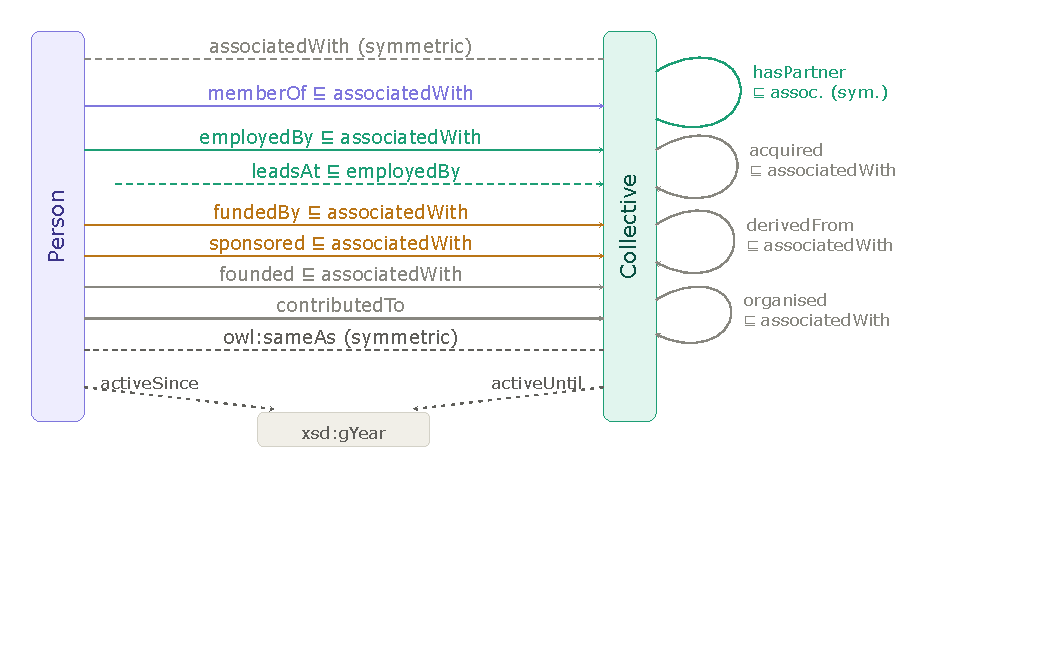
\includegraphics[trim={0 3.5cm 2cm 0.5cm},clip,width=\textwidth]{figures/lack-ontology-diagram.pdf}
    \vspace{-0.5cm}\caption{Schema diagram of the LACK ontology.}
\label{fig:ontology}\vspace{-0.5cm}
\end{figure}
\section{The LACK Knowledge Graph}
>>>>>>> 2cd6a84036c92e32b01883403f8af4ab7aa95d27
\label{sec:lack}

\vspace{-0.3cm}\paragraph{Sources.}
LACK was built from the two most comprehensive English-language databases dedicated to climate-lobbying actors\footnote{Pages accessed in December 2025.}.
The \textbf{DeSmog Climate Disinformation Database}~\cite{desmog}, maintained by DeSmog (an international investigative journalism organisation founded in 2006 and philanthropically funded), profiles individuals and organisations involved in climate denial, typically covering positions on climate science, affiliations, funding sources, and public statements; we collected all 943 profile pages.
\textbf{LobbyMap}~\cite{lobbymap}, maintained by InfluenceMap (an independent non-profit think tank founded in 2015), provides analyst-scored, IPCC-benchmarked assessments of corporate and industry-association engagement with climate policy for approximately 1{,}000 companies and 330 associations; we collected the 964 LobbyMap Scores profiles plus 338 further organisations referenced within them (1,302 pages total).
The two sources are complementary: DeSmog focuses on individuals and think tanks involved in disinformation, while LobbyMap covers groups engaging with policy; well-known actors appear in both.
The pages were collected using SPARQL Anything~\cite{daga2021opinionated}, querying DeSmog's HTML pages' index and the LobbyMap leaderboard JSON feed.

\begin{sloppypar}
\vspace{-0.3cm}\paragraph{Ontology.}
The LACK ontology (Figure~\ref{fig:ontology}) was designed bottom-up from the investigative sources: recurring information types were formalised as twelve competency questions (CQ1--CQ12), which drove the design of both the schema and the extraction process\footnote{\url{https://climatesense-project.eu/lack/ontology.html}}.
<<<<<<< HEAD
A guiding principle was to represent only what could be reliably and automatically extracted, deliberately excluding relation types (such as fine-grained roles) that could not be produced with sufficient confidence; this also motivated a purpose-built vocabulary, since general-purpose vocabularies such as Schema.org\footnote{\url{http://schema.org}} lack equivalents for lobbying-specific relations and would fragment the graph through intermediary role nodes.
The ontology defines two top-level classes, \texttt{lack:Person} (an individual) and \texttt{lack:Collective} (any group organised around a shared purpose, deliberately broad to accommodate events, journals, campaigns, and networks alongside organisations).
=======
The LACK ontology (Figure~\ref{fig:ontology}) was designed following the NeOn methodology~\cite{suarez2011neon}, with one deliberate adaptation: rather than eliciting requirements from domain experts directly, we treated the investigative sources themselves as a proxy for user needs, assuming that platforms such as DeSmog and LobbyMap already encode the questions their users care about.
To guide design, we derived twelve \textit{competency questions} (following~\cite{suarez2011neon}) from information content of the source pages, and re-engineered those sources, as non-ontological resources, into a domain schema\footnote{\url{https://climatesense-project.eu/lack/ontology.html}}; we revisit and confirm this assumption through the expert evaluation in Section~\ref{sec:evaluation}.
Practitioner requirements were not elicited at design time, so the schema is bounded by what the sources themselves document; the expert survey (Section~\ref{sec:eval:experts}) provides post-hoc validation and, as we discuss there, marks that boundary.
% The LACK ontology (Figure~\ref{fig:ontology}) was designed following the NeOn methodology~\cite{suarez2011neon}, combining a requirements specification expressed as twelve competency questions (CQ1--CQ12) with the re-engineering of our investigative sources, treated as non-ontological resources, into a domain schema\footnote{\url{https://climatesense-project.eu/lack/ontology.html}}.
% A guiding principle was to represent only what could be reliably and automatically extracted, 
Crucially, relation types that could not be derived from the sources are excluded.
We evaluated general-purpose vocabularies such as Schema.org~\cite{schemaorg} or the W3C Organisation ontology, which don't have lobbying-specific relations and/or would fragment the graph through intermediary role nodes.
The ontology defines two top-level classes, \texttt{lack:Person} (an individual) and \texttt{lack:Collective} (any group organised around a shared purpose, deliberately broad to accommodate events, journals, campaigns, and groups alongside organisations)\footnote{We note that alignments with \texttt{foaf:Agent} and \texttt{foaf:Person} are possible for \texttt{lack:Person} but not for \texttt{lack:Collective}.}.
>>>>>>> 2cd6a84036c92e32b01883403f8af4ab7aa95d27
Each relation is defined with a domain, range, and inverse, organised in a hierarchy rooted at the symmetric catch-all \texttt{lack:associatedWith}.
Relationships can be time-bounded, captured through entity-level bounds (\texttt{lack:activeSince}/\texttt{lack:activeUntil}) and relation-level annotations via reification~\cite{rdfprimer}, where each temporally annotated triple is reified as an \texttt{rdf:Statement} carrying \texttt{lack:since}/\texttt{lack:until}; reification was chosen over RDF-star for broad compatibility with current RDF tooling.
Provenance and source attribution reuse PROV-O~\cite{provo} and Dublin Core Terms~\cite{dcterms}, linking each statement to the extraction activity and to the source web page.\end{sloppypar}

<<<<<<< HEAD
\paragraph{Construction.}
The knowledge graph is produced from the raw extraction outputs by a pipeline implemented with SPARQL Anything~\cite{asprino2023knowledge}, reproducible from the source CSVs~\cite{lack-kgc}.
Relations are first extracted from the source pages by prompting Gemini 2.5 Flash~\cite{gemini25} with the allowed relation types and a strict JSON schema, then linked to authoritative identifiers through a hybrid entity-linking step combining Wikidata candidate retrieval, LLM-based disambiguation, and a web-search fallback, with Llama 3.3 70B~\cite{llama33} used at scale~\cite{lack-re,lack-el}.
Construction then proceeds in five phases: (i) the 152 distinct surface-form relation types (90,145 instances) are aligned to ontology properties; (ii) stable IRIs are minted per entity by hashing the highest-priority identifier available (Wikidata QID, then Wikipedia, then web page, then surface form with source URL), each typed as \texttt{lack:Person} or \texttt{lack:Collective} with a granular subtype and, where available, \texttt{owl:sameAs} links to Wikidata and DBpedia; (iii) each relation is written as a typed triple plus a reified statement carrying evidence and temporal bounds; (iv) PROV-O provenance is attached; and (v) ontology entailments (inverse pairs, sub-property promotions, symmetric closure) are materialised, growing the graph from 47,450 asserted relations to 188,862 triples.
=======
\vspace{-0.3cm}\paragraph{Construction.}
Relations are first extracted from the source pages by prompting Gemini 2.5 Flash~\cite{gemini25} with the allowed relation types and a strict JSON schema, then linked to authoritative identifiers through a hybrid entity-linking step combining Wikidata candidate retrieval, LLM-based disambiguation, and a web-search fallback, with Llama 3.3 70B~\cite{llama33} used at scale (see supplementary material~\cite{lack-re,lack-el}).
Construction encompasses five phases: (i) the 152 distinct surface-form relation types (90,145 instances) are aligned to ontology properties; (ii) stable IRIs are minted per entity by hashing the highest-priority identifier available (Wikidata QID, then Wikipedia, then web page, then surface form with source URL), each typed as \texttt{lack:Person} or \texttt{lack:Collective} with a granular subtype and, where available, \texttt{owl:sameAs} links to Wikidata and DBpedia; (iii) each relation is written as a typed triple plus a reified statement carrying evidence and temporal bounds; (iv) PROV-O provenance is attached; and (v) ontology entailments (inverse pairs, sub-property promotions, symmetric closure) are materialised, growing the graph from 47,450 \emph{asserted} relation triples, each evidenced by a source page, to 188,862 relation triples in total; the additional triples are entailed rather than independently extracted, and we keep the two counts separate throughout.
The knowledge graph is produced from the raw extraction outputs by a pipeline implemented with SPARQL Anything~\cite{sparqlanything} (reproducible at~\cite{lack-kgc}).
>>>>>>> 2cd6a84036c92e32b01883403f8af4ab7aa95d27

\vspace{-0.3cm}\paragraph{Availability and Maintenance.}
The LACK ontology and knowledge graph are published as Linked Open Data under a Creative Commons Attribution Non-Commercial 4.0 International (CC BY NC 4.0) licence.
Version 1.1 was released in April 2026 and is accessible at \url{https://climatesense-project.eu/lack/} as a Turtle dump (\texttt{KG.ttl}), a live SPARQL endpoint powered by QLever\footnote{\url{https://sparql.climatesense.kmi.tools/climatesense}}, and an interactive exploration interface.
Table~\ref{tab:kg-stats} summarises statistics; a full breakdown is on the LACK website.
The ontology is separately available under the persistent namespace \url{https://purl.net/climatesense/lack/ns#}, and the dataset is archived on Zenodo~\cite{lack}.
The resource is maintained by KMi and guaranteed available for at least five years under funder open data policy. 
Infrastructure for continuos updates is currently under development.
% \paragraph{Disclaimer.}
% LACK reorganises information from third-party investigative sources; the authors do not endorse or assume responsibility for the original claims, and the relations published surface structural connections rather than allegations against any named party.

\begin{table}[t]
\centering
\caption{LACK KG statistics. Inferred triples overlap with asserted ones, so the post-inference count is not their sum. The graph total additionally includes reified statements, provenance, and \texttt{owl:sameAs}/\texttt{rdfs:seeAlso} links.}
% \caption{Statistics. Inferred relation triples overlap with asserted ones (e.g.\ \texttt{associatedWith} may also be asserted), so the post-inference relation count is not their sum. Totals includes reified statements, provenance, and \texttt{owl:sameAs}/\texttt{rdfs:seeAlso}.}
\label{tab:kg-stats}
\small
\begin{tabular}{lr}
\toprule
\textbf{Dimension} & \textbf{Count} \\
\midrule
Entities (Person / Collective / Total)
  & 10,370 / 17,604 / \textbf{27,945} \\
\quad Wikidata links (Person / Collective / Total)
  & 2,911 / 5,369 / \textbf{8,280} \\
\quad DBpedia links (Person / Collective / Total)
  & 3,516 / 5,210 / \textbf{8,726} \\
\midrule
Relations triples, asserted          & 47,450 \\
Relations triples, after inference   & \textbf{188,862} \\
All triples in the graph     & \textbf{213,147} \\
Evidence (Desmog / LobbyMap / InfluenceMap / Total)
  & 943 / 964 / 338 / \textbf{2,245} \\
\bottomrule
\end{tabular}
\vspace{-0.5cm}
\end{table}

% \begin{table}[t]
% \centering
% \caption{LACK KG statistics.}
% \label{tab:kg-stats}
% \small
% \begin{tabular}{lr}
% \toprule
% \textbf{Dimension} & \textbf{Count} \\
% \midrule
% Entities (Person / Collective / Total)
%   & 10,370 / 17,604 / \textbf{27,945} \\
% \quad Wikidata links (Person / Collective / Total)
%   & 2,911 / 5,369 / \textbf{8,280} \\
% \quad DBpedia links (Person / Collective / Total)
%   & 3,516 / 5,210 / \textbf{8,726} \\
% \midrule
% Relations (Asserted / Inferred / Total)
%   & 47,450 / 142,737 / \textbf{213,147} \\
% Evidence (Desmog / LobbyMap / InfluenceMap / Total)
%   & 943 / 964 / 338 / \textbf{2,245} \\
% \bottomrule
% \end{tabular}
<<<<<<< HEAD
% \end{table}
=======
% \end{table}
>>>>>>> 2cd6a84036c92e32b01883403f8af4ab7aa95d27
